Na tomto projektu jsem začal pracovat asi dva týdny po příchodu do firmy. Uměl jsem jen HTML, CSS, základy JavaScriptu a díky dvou týdnům převádění Less stylů na Sass jsem měl určité povědomí o struktuře repozitáře. Stále jsem ale nerozuměl Reactu, Next.js, Storybooku, ani ostatním technologiím, o kterých jsem v předchozí kapitole psal. Proto bylo rozhodnuto, že bude nejlepší se tyto technologie naučit. A volba padla právě na stránku s nastavením účtem.

Bylo to ideální. Šlo o poslední stránku (kromě administrace, která je ale samostatný projekt sama o sobě) napsanou v českém Nette frameworku. Nette renderuje stránky na serveru, což snižuje jejich interaktivitu, nepodporuje SPA a celkově si moc s React ekosystémem nerozumí\cite{NetteHowAppsWork}. Navíc se s přechodem na Next.js a Sass styly stránky částečně rozbily, a než ji stále kontrolovat a opravovat, bylo lepší zbavit se technického dluhu a~konečně ji přepsat.

\begin{figure}[!h]
    \centering
    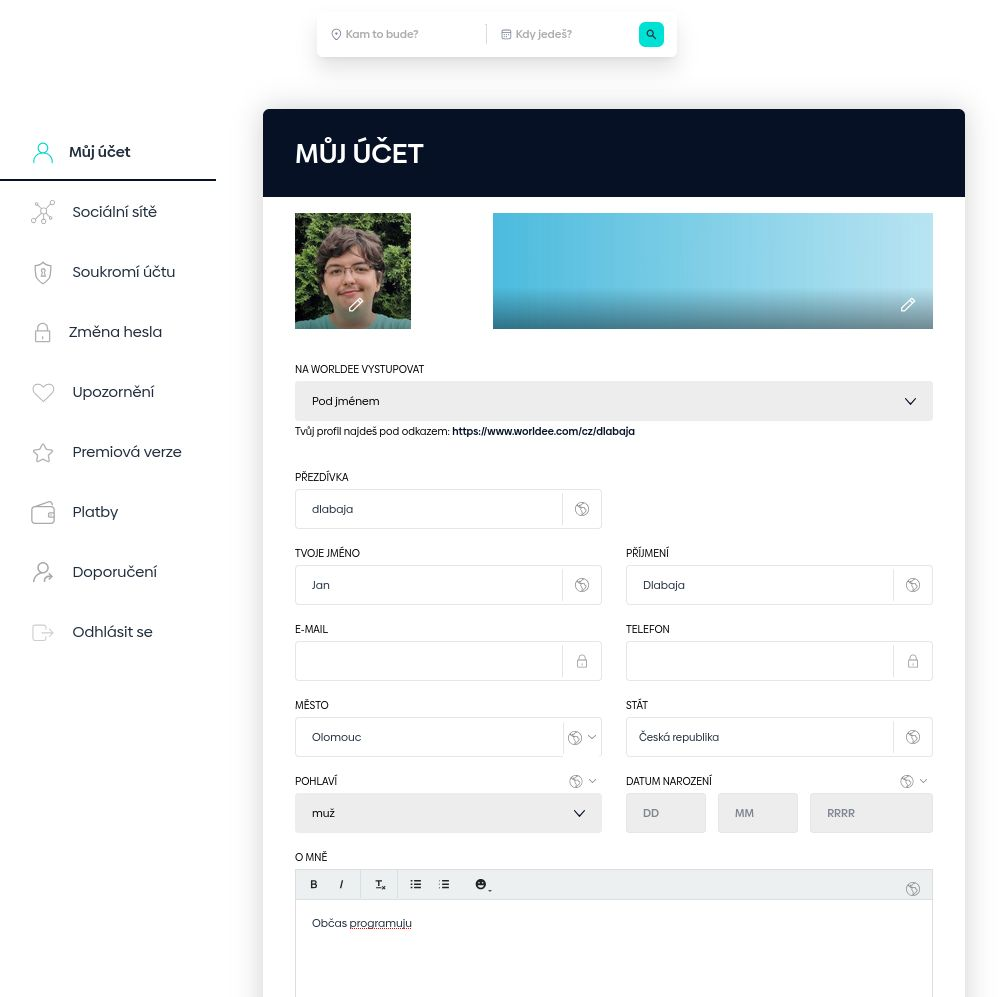
\includegraphics[width=0.7\linewidth]{obrazky/settings_old.png}
    \caption{Staré nastavení účtu napsané v Nette. Zdroj: vlastní práce.}
\end{figure}